\documentclass[final,3p,times,10pt,onecolumn]{myElsarticle}
\usepackage{float}
\usepackage{times}
\usepackage[utf8]{inputenc}
\usepackage[english]{babel}
\usepackage[T1]{fontenc}
\usepackage{geometry}
\usepackage{color}
\usepackage{soul}
\usepackage{cancel}
\usepackage{subfigure}
\usepackage{enumerate}
\usepackage{amsmath,amsthm,amsfonts,amssymb}
\usepackage{amsthm}
\usepackage{graphicx}
\graphicspath{{./figs/}}
\numberwithin{equation}{section}
\usepackage{spverbatim}
\usepackage{fancyhdr}
\usepackage{listings} 
\usepackage{lineno}
\usepackage[none]{hyphenat}
\date{\today}
\setcounter{secnumdepth}{3}
\providecommand{\abs}[1]{\lvert#1\rvert}
\providecommand{\norm}[1]{\lVert#1\rVert}
\setlength\parindent{12pt}		

\linenumbers

\newcommand{\COM}[1]{{\color{green} #1}}
\newcommand{\HA}[1]{{\color{red} #1}}
\newcommand{\CIP}[1]{{\color{blue} #1}}
\newcommand{\CMV}[1]{{\color{orange} #1}}


\begin{document}

\begin{frontmatter}

\title{A second-order approximation on SIMPLEC: the COMPLEX algorithm}
%% A second-neighbor extended correction for segregated p-v coupling algorithms
 
\author[a,e]{Horacio J. Aguerre}
\author[b,a]{Cesar I. Pairetti}
\author[a,b]{Cesar M. Venier}
\author[a,c]{Santiago Marquez Damian}
\author[a,d]{Norberto M. Nigro}

\address[a]{Centro de Investigación de Métodos Computacionales, CONICET-UNL, Santa Fe, Argentina}
\address[b]{Escuela de Ingenier\'ia Mec\'anica, Facultad de Ciencias Exactas, Ingenieria y Agrimensura, Universidad Nacional de Rosario, Rosario, Argentina}
\address[c]{Facultad Regional Santa Fe, Universidad Tecnologica Nacional, Santa Fe, Argentina}
\address[d]{Facultad de Ingeniería y Ciencias Hídricas, Universidad Nacional del Litoral, Santa Fe, Argentina}
\address[e]{Facultad Regional Concepción de Uruguay, Universidad Tecnologica Nacional, Concepción del Uruguay, Argentina}

%Start of abstract
\begin{abstract}
In this paper, we present an enhancement of the segregated SIMPLE-like algorithms.

\CIP{Con estos comandos podemos hacer comentarios que después vayamos a borrar}

\end{abstract}

\begin{keyword}
Segregated algorithms \sep Segregated method \sep Collocated grids \sep Finite Volume Method 
\end{keyword}
\end{frontmatter}

\section*{Graphical abstract}
\begin{figure}[h]
\centering
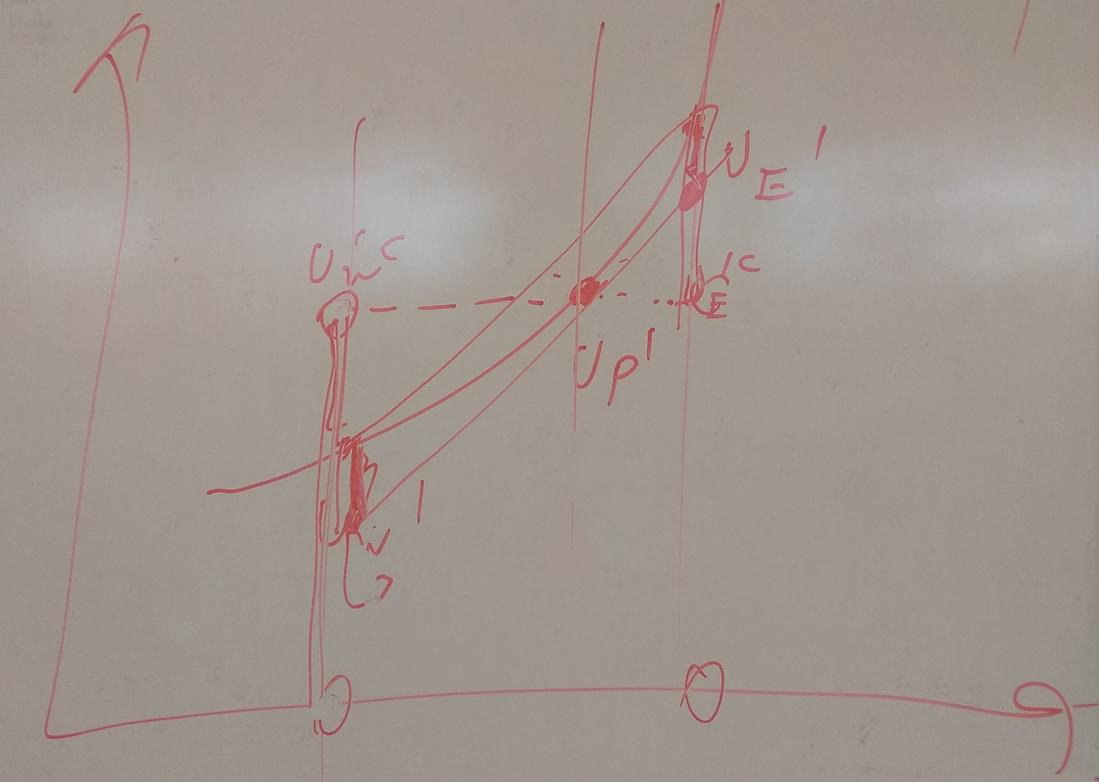
\includegraphics[width=8cm]{graph_abstract.jpg}
\end{figure}

%%%%%%%%%%%%%%%%%%%%%%%%%%%%%%%%%%%%%
\section{Introduction}
%In the context of the Finite Volume Method (FVM), segregated algorithms are among the most popular strategies to couple pressure and velocity in Computational Fluid Dynamics (CFD). In these methodologies, the variables of the problem can be stored in the same or different spatial location, which gives place to grid arrangements known as collocated or staggered  respectively. The staggered grids have the advantage of avoiding interpolations and thus prevents the appearance of spurious oscillations on the unknown fields. On the other hand, collocated grid arrangements are more suitable for unstructured meshes which are mandatory to address practical applications involving complex geometries.

%\COM{Acá va un review de los algoritmos segregados: SIMPLE ... IDEAL. Ver papes Xiao y Liu. \\ A continuación hay un extracto de la introducción del paper de Fourier}

The SIMPLE family techniques 
\cite{patankar1972, patankar1981, vanDoormal, tao, tao2, cheng, issa} are arguably the most 
widely used pressure-based algorithms to iteratively couple the pressure and 
velocity fields for incompressible flows in CFD codes nowadays \cite{patankar1980,
moukalled,ferziger,versteeg,weller,fluent}. The pioneering SIMPLE algorithm of Patankar 
and Spalding \cite{patankar1972} rely on decoupling the calculation of the pressure and velocity fields. 
First, an approximation of the velocity field is obtained based on the momentum equation. Then, an equation 
for the pressure is assembled based on the continuity equation and an explicit velocity expression obtained 
from the momentum equation. This expression neglects the neighbor velocity corrections contribution which 
may induce instabilities in the coupling algorithm. The method concludes by solving the pressure field and an 
updating the velocity field using the explicit expression previously mentioned. This sequence is iterated 
until a certain convergence criteria is fulfilled. In order to enhance the stability of the method, under-
relaxation factors are usually employed for the pressure field and the momentum equation. Among them, the 
SIMPLER algorithm \cite{patankar1981} was conceived as a way to enhance the rate of convergence 
of the standard SIMPLE algorithm by computing a pressure field 
separately from the velocity correction sequence. Later on, 
Van Doormaal and Raithby \cite{vanDoormal} developed the SIMPLEC 
method, which avoids the pressure 
under-relaxation by manipulating diagonal and off-diagonal 
coefficients of the momentum equation to assemble 
the pressure equation. All these methods were originally 
developed to 
address steady state \COM{hydrodynamics} and later extended to 
time-marching problems employing several 
iterations per time step. In contrast, the PISO algorithm 
\cite{issa} was originally conceived as a low-cost transient 
flow solver, which presents 
the particular feature of introducing several corrections to 
\COM{enforce the pressure-velocity coupling at each time step.}

\CIP{En los trabajos anteriores analizamos PISO porque queremos hacer transitorio y lo evaluamos con Fourier. Para este trabajo habría que extender el review anterior sobre las mejoras de SIMPLE, explicando por qué se hicieron y por qué nosotros queremos mejorarlo aún más.}


This work propose \CIP{a slight modification on the SIMPLEC formulation, particularly in the \textit{a priori} approximation of neighbor values, that enhance the convergence of the algorithm significantly}.

The paper is organized as follows: On Section \ref{sec:theory}, the standard SIMPLE (Semi-Implicit Method for Pressure-Linked Equations) is given, explaining how SIMPLEC enhance its performance. Section \ref{sec:COMPLEX} presents an extension of the SIMPLEC approach using second-order approximations for neighbours values. In Section \ref{sec:cases}, \COM{X} benchmark cases are solved to evaluate the efficiency of the algorithms. The conclusions of this study are presented in the last section.


\section{Theoretical background} \label{sec:theory}

\subsection{The SIMPLE algorithm on collocated grids}

The continuum incompressible Navier-Stokes equations may be presented as:

\begin{equation}
\displaystyle \nabla \cdotp \boldsymbol{u} = 0, 
\label{eq:mass1}
\end{equation}

\begin{equation}
\displaystyle \frac{\partial \boldsymbol{u}}{\partial t} + \nabla \cdotp (\boldsymbol{u} \boldsymbol{u}) = -\nabla p + \nu\, \nabla^2 \boldsymbol{u} + \boldsymbol{\Phi},
\label{eq:mom1}
\end{equation}

\noindent where $\displaystyle p = \frac{\mathcal{P}}{\rho}$, $\mathcal{P}$ is the pressure field, $\boldsymbol{u} = (u,v,w)$ is the velocity field, {\color{red}$\rho$ is the mass density, }$\nu$ is the kinematic viscosity and $\mathbf{\Phi}$ is a momentum source term (e.g. a body force).
Based on the Finite Volume Method \cite{jasak}, Eqs.~(\ref{eq:mass1}) and~(\ref{eq:mom1}) may be discretized as:

\begin{equation}
\begin{split}
\sum_{f} \boldsymbol{u}_{f} \cdotp \textbf{S}_{f} = \sum_{f} F_f = 0, 
\end{split}
\label{eq:mass2} 
\end{equation}

\begin{equation}
\begin{split}
a_P\,\boldsymbol{u}_P + \sum_{N} a_{N}\,\boldsymbol{u}_{N} = b_P\, \boldsymbol{u}^0_P + \boldsymbol{\Phi}_P - \nabla p_P,
\label{eq:umom1}
\end{split}
\end{equation}

\noindent where the subscript $P$ indicates the cell-centered value of the current cell, $N$ indicates neighbor cells values and $f$ refers to the face values. The term ${\color{red}b_P}\, \boldsymbol{u}^0_P$ is the contribution of the previous time-step and is function of the temporal scheme. {\color{red} The face-normal vector $\textbf{S}_{f}$ has the magnitude of the face area and points out of the cell}, $F_f$ is the {\color{red} velocity} flux at the face $f$ and $a_P$ and $a_{N}$ are the diagonal and off-diagonal momentum matrix coefficients respectively. The operator $\nabla p_P$ is a Gauss-based gradient of the pressure computed using first neighbors values of that field. Isolating $\boldsymbol{u}_P$ from Eq.~(\ref{eq:umom1}),

\begin{equation}
\begin{split}
\boldsymbol{u}_P = \frac{1}{a_P}\left(b_P\, \boldsymbol{u}^0_P + \boldsymbol{\Phi}_P - \sum_{N} a_{N}\, \boldsymbol{u}_{N} - \nabla p_P\right),
\label{eq:uP}
\end{split}
\end{equation}

One way to solve Eqs. (\ref{eq:mass2}) and (\ref{eq:umom1}) for $\boldsymbol{u}$ and $p$ consists on addressing one equation at a time, update one of the unknown fields, solve the remaining equation and iterate the sequence. These techniques are known as segregated methods, where the SIMPLE-family techniques \cite{patankar1972,patankar1980,patankar1981,vanDoormal,issa} are among the most popular for incompressible flows. It broadly consists of a Momentum Predictor step and a Corrector step. In the Momentum Predictor, a first approximation for the velocity field is computed using the momentum equation where the pressure term is treated explicitly. 
{\color{red}
\begin{equation} \label{eq:MOMPRED}
\begin{split}
a_P\, \boldsymbol{u}_P^{*} = \boldsymbol{H}^* - \nabla p_P^{*}%, \\
%p_P^* &= p_P^0
\end{split}
\end{equation}

\CIP{En este punto podríamos meter la definición de H si es que queremos escribir todo "a la FOAM". Me parece más natural escribir en términos de $u$, así se ve más claro cómo entra la aproximación de los vecinos usando el gradiente de velocidad}

\noindent where 

\begin{equation}
\boldsymbol{H}^* = - \sum_N a_N \boldsymbol{u}_N^* + \boldsymbol{\Phi}_P    
\end{equation}

\noindent and the superscript $0$ indicates fields that are stored from previous iterations and $*$ are the fields being solved at the current iteration. }
This preliminary result does not satisfy the divergence-free condition in Eq. (\ref{eq:mass2}). In the Corrector step, a pressure correction is computed from an equation based on including the momentum equation, as expressed in Eq. (\ref{eq:uP}), in the mass conservation  Eq. (\ref{eq:mass2}). In this context, the velocity correction can be expressed in the following manner

\CIP{A continuación desarrollo las ecuaciones de forma relativa. Hay que definir si queda así o en términos absoultos (como FOAM). La ventaja del $H$ es que Rhie Chow queda implícito (acá no está hecho) y que FOAM labura así.}

\begin{align}
\label{eq:uprimeDef}
\boldsymbol{u}_P^{**} &= \boldsymbol{u}_P^{*} + \boldsymbol{u}_P^{'} \\
\qquad \boldsymbol{u}_P^{'} &= \frac{1}{a_P}\left(\boldsymbol{H}'- \nabla p_P^{'}\right).
\end{align}

\noindent where,

\begin{align}
\label{eq:HPrima}
   \boldsymbol{H}' = - \sum_N a_N \boldsymbol{u}'_N 
\end{align}

Then, the divergence-free condition can be expressed in terms of the previous expressions

\begin{align} \label{eq:div-free1}
\nabla \cdot \left(\boldsymbol{u}_P^{*} + \boldsymbol{u}_P^{'}\right) &= 0 \\
\sum_f \left(\boldsymbol{u_P}'\right)_{f} \cdot \boldsymbol{S}_f &= -\sum_f \left(\boldsymbol{u_P}^{*}\right)_{f} \cdot \boldsymbol{S}_f \label{eq:div-free2} \\
\sum_f \left[\frac{1}{a_P}\left(\boldsymbol{H}' - \nabla p_P^{'}\right)\right]_f\cdot \boldsymbol{S}_f &= -\sum_f \left[\frac{1}{a_P}\left(\boldsymbol{H}^* - \nabla p_P^{*}\right)\right]_f \cdot \boldsymbol{S}_f \label{eq:div-free3}
\end{align}

%\noindent where, $\boldsymbol{u}^*_f$ is obtained by linear interpolation of the $\boldsymbol{u}^*_{P}$ values on the cells that shares the same face $f$.

%The system of equations given by \ref{eq:div-free} for all the cells is highly coupled due to the presence of the corrections on the neighbors. To reduce the computational effort, the SIMPLE algorithm introduce the assumption that $\boldsymbol{u}'_N$ are negligible. With this simplification, the system turns to be

The SIMPLE method considers $\boldsymbol{H}'=\boldsymbol{0}$, thus Eq.~(\ref{eq:div-free2}) becomes:

\begin{equation}
\sum_f 
\left[
\frac{1}{a_P}
\left(
-
\nabla p_P^{'}
\right)
\right]_f\cdot \boldsymbol{S}_f 
=
-\sum_f \left[\frac{1}{a_P}\left(\boldsymbol{H}^* - \nabla p_P^{*}\right)\right]_f \cdot
\boldsymbol{S}_f.
\label{eq:div-free4}    
\end{equation}
Then, grouping the pressure terms, a relation based on $p^{**}$ is obtained,
\begin{equation}
\sum_f 
\left[
\frac{1}{a_P}
\left(
\nabla p_P^{**}
\right)
\right]_f\cdot \boldsymbol{S}_f 
=
\sum_f 
\left[
\frac{1}{a_P}
\left(
\boldsymbol{H}^*
\right)
\right]_f
\cdot
\boldsymbol{S}_f.
\label{eq:div-free5}  
\end{equation}

% \begin{equation}
% \label{eq:pEqnSIMPLE1}
% \sum_f \left(\frac{1}{a_P}\right)_f \nabla p_f^{'}  \cdot \boldsymbol{S}_f= \sum_f \left[\frac{1}{a_P}\left(\boldsymbol{H}^* - \nabla p_P^{*}\right)\right]_f \cdot \boldsymbol{S}_f
% \end{equation}

% (acá hay que escribir algun bolazo de porque distribuimos la interpolación en el producto)

\noindent which is a Poisson problem that has the pressure correction values as unknowns. Nevertheless, solving this system in a straightforward manner may lead to high-frequency oscillations. The Rhie-Chow correction \cite{rhiechow} reduces this effect in collocated grids, 

\begin{equation}
\label{eq:pEqnSIMPLE2}
\sum_f 
\left[
\frac{1}{a_P}
\left(
\nabla p_P^{**}
\right)
\right]_f\cdot \boldsymbol{S}_f 
=
\sum_f 
\left[
\frac{1}{a_P}
\left(
\boldsymbol{H}^*
\right)
\right]_f
\cdot
\boldsymbol{S}_f 
+
\sum_f  
\left[
\left(
\frac{\nabla p_P^{**}}{a_P}
\right)_f
- 
\left(
\frac{1}{a_P}
\right)_f 
\nabla p_f^{**} 
\right]
\cdot 
\boldsymbol{S}_f 
\end{equation}

 Finally, the pressure equation can be written as:



\begin{equation}\label{eq:pEqnSIMPLE3}
\sum_f \left(\frac{1}{a_P}\right)_f \nabla p_f^{**} \cdot \boldsymbol{S}_f =  \sum_f \left(\frac{\boldsymbol{H}^*}{a_P}\right)_f \cdot \boldsymbol{S}_f 
\end{equation}

\noindent where,

\begin{equation}
 p_P^{'} = p_P^{**} - p_P^{*}
\end{equation}

The corrected velocity value is then given by

\begin{equation}\label{eq:SIMPLECorr}
\boldsymbol{u}_P^{**} = \boldsymbol{u}_P^* - \frac{\nabla p_P'}{a_P}.
\end{equation}

\iffalse
 In order to do so, the velocity field $\boldsymbol{u}_P$, originally on cell-centers, needs to be interpolated to the faces obtaining: 

 \begin{equation}
 \begin{split}
 \sum_{f} \left( \boldsymbol{H}_P - \frac{1}{a_P} \nabla p_P  \right)_f \cdotp \textbf{S}_{f} = 0 
 \end{split}
 \label{eq:pEq1} 
 \end{equation}

Therefore, the Corrector step may be summarized as:

\begin{enumerate}

\item Assemble and solve the pressure based on Eq.~(\ref{eq:pEq1}):

\begin{equation}
\begin{split}
\sum_{f} \left( \frac{1}{a_P} \nabla p'_P \right)_f \cdotp \textbf{S}_{f} = \sum_{f} \boldsymbol{u}^*_f \cdotp \textbf{S}_{f}
\end{split}
\label{eq:pEq2} 
\end{equation}


%\CIP{Si conservamos la forma relativa, aquí habría que meter la explicación de Rhie Chow}

\item {\color{red}Compute} the face fluxes by adding the new pressure contribution:

\begin{equation}
\begin{split}
F_f = \boldsymbol{u}^*_f \cdotp \textbf{S}_{f} -  \left( \frac{1}{a_P}\right)_f \nabla p'_f  \cdotp \textbf{S}_{f}
\end{split}
\label{eq:Fhat} 
\end{equation}

\item Correct the cell-centered velocity field based on the new pressure field, using Eq. (\ref{eq:umom3b})

\begin{equation}\label{eq:umom3b}
\begin{split}
\boldsymbol{u}_P = \boldsymbol{u}^*_P - \frac{1}{a_P} \nabla p'_P 
\end{split}
\end{equation}

\end{enumerate}

\fi
Most of the SIMPLE-family algorithms preserve this general structure. In particular, the SIMPLE algorithm \cite{patankar1972}, originally conceived as a steady state flow solver, adds under-relaxation factors to obtain a stable solution. Another variant is the PISO {\color{red}(Pressure-Implicit with Splitting of Operators)} algorithm, which relies on iterating the Corrector step a given number of times to ensure a correct coupling between pressure and velocity for transient flow problems \cite{issa,issa2}. {\color{red} The SIMPLE-PISO combined technique has been largely adopted in several computational codes (e.g. OpenFOAM(R) \cite{ofpg}) to address transient incompressible flow problems due to its beneficial convergence features. It consists on iterating the corrector steps until a certain mass conservation criteria is fulfilled (as in PISO) and iterating the whole sequence (Momentum Predictor and Corrector Step) several times until both mass and momentum equations are verified for each time step. This algorithm will be adopted in the present work.}

\subsection{Improving the neighbor approximation: the SIMPLEC algorithm}
The SIMPLEC~\cite{vanDoormal} algorithm proposes an aproximation of the neighbour velocity correction $\boldsymbol{u}_N'$,
\begin{equation}
\label{Eq:simplecAproximation}
\boldsymbol{u}_N'
=
\boldsymbol{u}_P'
\end{equation}
Based on last assumption the Eq.~(\ref{eq:HPrima}) may be expressed as,

\begin{equation}\label{eq:H_SIMPLEC}
\boldsymbol{H}'= \left(-\sum_N a_N\right) \boldsymbol{u}'_P,
\end{equation}

\noindent which can be computed and included in the momentum equation leading to:

\begin{align}\label{eq:uPrimeSIMPLEC}
a_P\,\boldsymbol{u}_P^{'} &= -\boldsymbol{u}'_P \sum_{N} a_{N}\ - \nabla p_P^{'}
\end{align}

\noindent and then

\begin{align}\label{eq:uPrimeSIMPLEC2}
 \boldsymbol{u}_P^{'} &= - \frac{\nabla p_P^{'}}{a_P + \sum_{N} a_{N}}
\end{align}


The following equivalence is defined,
\begin{equation}
\tilde{a}_p 
\equiv
a_P + \sum_{N} a_{N},
\end{equation}
Then:

\begin{align}\label{eq:uPrimeSIMPLEC2}
\boldsymbol{u}_P^{'} 
=
- 
\dfrac
{
\nabla p_P^{'}
}
{
\tilde{a_P}
}
\end{align}

Including this expression into Eq.~(\ref{eq:div-free2}):

\begin{align} 
\sum_f \left(\boldsymbol{u_P}'\right)_{f} \cdot \boldsymbol{S}_f &= -\sum_f \left(\boldsymbol{u_P}^{*}\right)_{f} \cdot \boldsymbol{S}_f \label{eq:div-free4}
\end{align}
\noindent the following pressure equation is obtained:

\begin{equation}
\label{eq:pEqnSIMPLEC1}
\sum_f 
\left[
\left(
\frac
{
1
}
{
\tilde{a}_P
}
\right)
\nabla p_P^{'}
\right]_f
\cdot 
\boldsymbol{S}_f
= 
\sum_f 
\left[
\frac{1}{a_P}
\left(
\boldsymbol{H}^* - \nabla p_P^{*}
\right)
\right]_f 
\cdot
\boldsymbol{S}_f.
\end{equation}


Adding the following term  in both terms of previous equation
\begin{equation}
\sum_f
\left[
\left(
\dfrac
{1}
{\tilde{a}_P}
\right)
\nabla p^*
\right]_f
 \cdot S_f,
\end{equation}
 and grouping the pressure terms,
\begin{equation}
\label{eq:pEqnSIMPLEC1}
\sum_f 
\left[
\left(
\frac
{
1
}
{
\tilde{a}_P
}
\right)
\nabla p_P^{**}
\right]_f
\cdot 
\boldsymbol{S}_f
= 
\sum_f 
\left[
\frac{1}{a_P}
\left(
\boldsymbol{H}^*
\right)
\right]_f 
\cdot
\boldsymbol{S}_f
+
\sum_f
\left[
\left(
\dfrac{1}
{\tilde{a}_P}
-
\dfrac{1}
{a_P}
\right)
\nabla p^*
\right]_f
\cdot
\boldsymbol{S}_f
\end{equation}


The pressure equation is obtained by including an analogous Rhie-Chow correction:

\begin{equation}
\begin{split}
\label{eq:pEqnSIMPLEC2}
\sum_f 
\left[
\left(
\frac
{
1
}
{
\tilde{a}_P
}
\right)
\nabla p_P^{**}
\right]_f
\cdot 
\boldsymbol{S}_f
=
\\ 
\sum_f 
\left[
\frac{1}{a_P}
\left(
\boldsymbol{H}^*
\right)
\right]_f 
\cdot
\boldsymbol{S}_f
+
\sum_f
\left[
\left(
\dfrac{1}
{\tilde{a}_P}
-
\dfrac{1}
{a_P}
\right)
\nabla p^*
\right]_f
\cdot
\boldsymbol{S}_f
+
\sum_f
\left\lbrace
\left(
\dfrac
{
\nabla p^{**}
}
{\tilde{a}_P}
\right)_f
-
\left(
\dfrac
{1}
{\tilde{a}_P}
\right)_f
\nabla p^{**}_f
+
\left(
\dfrac
{1}
{\tilde{a}_P}
-
\dfrac
{1}
{a_P}
\right)_f
\nabla p^{*}_f
-
\left[
\left(
\dfrac
{1}
{\tilde{a}_P}
-
\dfrac
{1}
{a_P}
\right)
\nabla p^*
\right]_f
\right\rbrace
\cdot
S_f
\end{split}
\end{equation}
Then, simplifying,
\begin{equation}
\sum_f
\left[
\left(
\dfrac
{1}
{\tilde{a}_P}
\right)_f
\nabla p^{**}_f
\right]
\cdot 
\boldsymbol{S}_f
= 
\sum_f 
\left[
\frac{1}{a_P}
\left(
\boldsymbol{H}^*
\right)
\right]_f 
\cdot
\boldsymbol{S}_f
+
\sum_f
\left[
\left(
\dfrac
{1}
{\tilde{a}_P}
-
\dfrac
{1}
{a_P}
\right)_f
\nabla p^{*}_f
\right]
\cdot
\boldsymbol{S}_f
\end{equation}


Then, the velocity correction may be computed as follows:

\begin{equation}\label{eq:uCorrSIMPLEC}
\boldsymbol{u}^{**}_P = \boldsymbol{u}_P^* - \frac{\nabla p_P^{'}}{\tilde{a}_P}.
\end{equation}

Last equation may be expressed also by means of the $H^*$ operator,
\begin{equation}
\boldsymbol{u}^{**}_P 
=
\dfrac
{\boldsymbol{H}_P^* }
{a_P}
- 
\frac{\nabla p_P^{*}}{a_P}
- 
\frac{\nabla p_P^{'}}{\tilde{a}_P}.
\end{equation}
which may be considered including absolute pressure values,
\begin{equation}
\boldsymbol{u}^{**}_P 
=
\dfrac
{\boldsymbol{H}_P^* }
{a_P}
- 
\frac{\nabla p_P^{**}}{\tilde{a}_P}
+
\left(
\dfrac{1}{\tilde{
a}_P}
-
\dfrac{1}{a_P}
\right)
\nabla p_P^{*}.
\end{equation}


The only difference between SIMPLE and SIMPLEC are the coefficients in the Corrector step. Nevertheless, this slight modification shows a significant improvement in the stability  and convergence properties of the algorithm \cite{liu}. In the spirit of using better approximation for the neighbors correction values, we propose the following method.

\section{Enhancement of SIMPLEC: the COMPLEX method}
\label{sec:COMPLEX}

In order to estimate the value of $\boldsymbol{u}_N'$ in Eq.~(\ref{eq:HPrima}), a second order Taylor approximation is proposed,
\begin{equation}\label{eq:uNTaylor}
\boldsymbol{u}_N' = \boldsymbol{u}_P' + \boldsymbol{x}_{PN}\cdot 
\nabla \boldsymbol{u}_f'.
\end{equation}

Replacing Eq.~(\ref{eq:uNTaylor}) in (\ref{eq:HPrima}), considering the same velocity gradient for all the neighbor approximations
\begin{align}
\label{eq:uPrimeCOMPLEX}
a_P\,\boldsymbol{u}_P^{'} 
&=
 -\sum_{N} a_{N}\, \left(\boldsymbol{u}_P^{'} + \boldsymbol{x}_{PN}\cdot \nabla \boldsymbol{u}_f'\right)- \nabla p_P^{'}, 
\\
\boldsymbol{u}_P^{'} 
&=
- \dfrac{\nabla p_P^{'}}
{\tilde{a}_P}
-
\dfrac
{
\sum_{N} a_{N} 
( 
\boldsymbol{x}_{PN} 
\cdot
\nabla \boldsymbol{u}_f' 
)
}
{\tilde{a}_P}.
\end{align}

\begin{align} 
\label{eq:div-free4Again}
\sum_f \left(\boldsymbol{u_P}'\right)_{f} \cdot \boldsymbol{S}_f &= -\sum_f \left(\boldsymbol{u_P}^{*}\right)_{f} \cdot \boldsymbol{S}_f 
\end{align}

\begin{equation}
\label{eq:pEqnCOMPLEX1}
\sum_f 
\left[
\left(
\frac
{
1
}
{
\tilde{a}_P
}
\right)
\nabla p_P^{'}
\right]_f
\cdot 
\boldsymbol{S}_f
= 
\sum_f 
\left[
\frac{1}{a_P}
\left(
\boldsymbol{H}^* - \nabla p_P^{*}
\right)
\right]_f 
\cdot
\boldsymbol{S}_f
-
\sum_f 
\left[
\dfrac
{
\sum_{N} a_{N} 
( 
\boldsymbol{x}_{PN} 
\cdot
\nabla \boldsymbol{u}_f' 
)
}
{\tilde{a}_P}
\right]_f 
\cdot
\boldsymbol{S}_f.
\end{equation}

\begin{equation}
\label{Eq:complexSemiFinal}
\sum_f
\left[
\left(
\dfrac
{1}
{\tilde{a}_P}
\right)_f
\nabla p^{**}_f
\right]
\cdot 
\boldsymbol{S}_f
= 
\sum_f 
\left[
\frac{1}{a_P}
\left(
\boldsymbol{H}^*
\right)
\right]_f 
\cdot
\boldsymbol{S}_f
+
\sum_f
\left[
\left(
\dfrac
{1}
{\tilde{a}_P}
-
\dfrac
{1}
{a_P}
\right)_f
\nabla p^{*}_f
\right]_f
\cdot
S_f
-
\sum_f 
\left[
\dfrac
{
\sum_{N} a_{N} 
( 
\boldsymbol{x}_{PN} 
\cdot
\nabla \boldsymbol{u}_f' 
)
}
{\tilde{a}_P}
\right]_f 
\cdot
\boldsymbol{S}_f
\end{equation}

\subsection{Computation of the face gradient}
To define the face gradient $\boldsymbol{u}_f$, the face values $\boldsymbol{u_P}'_f$ of the mass balance of Eq.~(\ref{eq:div-free4Again}) are expressed as a  first-order Taylor expansion  using $\boldsymbol{u}_f$,
\begin{equation}
\label{Eq:TaylorOnFace}
\left(
\boldsymbol{u_P}'
\right)_f
=
\boldsymbol{u_P}'
+
\boldsymbol{x}_{Pf}
\cdot 
\nabla \boldsymbol{u}_P'.
\end{equation} 
Subsequently, this last equation is replaced in  Eq.~(\ref{eq:div-free4Again}),
\begin{align}
\sum_f 
\left(
\boldsymbol{u_P}'
+
\boldsymbol{x}_{Pf}
\cdot 
\nabla \boldsymbol{u}_P'
\right)
\cdot 
\boldsymbol{S}_f 
&=
-\sum_f
\left(
\boldsymbol{u_P}^{*}
\right)_{f} 
\cdot 
\boldsymbol{S}_f
\\
\boldsymbol{u_P}'
\cdot 
\sum_f 
\boldsymbol{S}_f
+
\sum_f 
\left(
\boldsymbol{x}_{Pf}
\cdot 
\nabla \boldsymbol{u}_P'
\right)
\cdot 
\boldsymbol{S}_f
&=
-\sum_f
\left(
\boldsymbol{u_P}^{*}
\right)_{f} 
\cdot 
\boldsymbol{S}_f
\\
\label{Eq:Last}
\sum_f 
\left(
\boldsymbol{x}_{Pf}
\cdot 
\nabla \boldsymbol{u}_P'
\right)
\cdot 
\boldsymbol{S}_f
&=
-\sum_f
\left(
\boldsymbol{u_P}^{*}
\right)_{f} 
\cdot 
\boldsymbol{S}_f
\end{align}

where,
\begin{equation}
\left(
\boldsymbol{u_P}^{*}
\right)_{f}
=
\left[\frac{1}{a_P}\left(\boldsymbol{H}^* - \nabla p_P^{*}\right)\right]_f
\end{equation}

Then, a similar form of the Rhie-Chow term given in Eq.~(\ref{eq:pEqnSIMPLE2}) is included,
\begin{equation}
\left(
\boldsymbol{u_P}^{*}
\right)_{f}
=
\left[\frac{1}{a_P}\left(\boldsymbol{H}^* - \nabla p_P^{*}\right)\right]_f
+
\left[
\left(
\frac{\nabla p_P^{*}}{a_P}
\right)_f
- 
\left(
\frac{1}{a_P}
\right)_f 
\nabla p_f^{*} 
\right]
\end{equation}

Simplifying, 
\begin{equation}
\left(
\boldsymbol{u_P}^{*}
\right)_{f}
=
 \left(\frac{\boldsymbol{H}^*}{a_P}\right)_f 
 -
 \left(\frac{1}{a_P}\right)_f \nabla p_f^{*}
\end{equation}

Replacing in Eq.~(\ref{Eq:Last}),
\begin{equation}
\sum_f 
\left(
\boldsymbol{x}_{Pf}
\cdot 
\nabla \boldsymbol{u}_P'
\right)
\cdot 
\boldsymbol{S}_f
=
-\sum_f
\left[
\left(\frac{\boldsymbol{H}^*}{a_P}\right)_f 
 -
 \left(\frac{1}{a_P}\right)_f \nabla p_f^{*}
 \right]
\cdot 
\boldsymbol{S}_f
\end{equation}
The following assumption is proposed:
\begin{equation}
\nabla \boldsymbol{u}_P'
=
\alpha
\boldsymbol{I}
\end{equation}

Replacing,
\begin{align}
\sum_f 
\left(
\boldsymbol{x}_{Pf}
\cdot 
\alpha
\boldsymbol{I}
\right)
\cdot 
\boldsymbol{S}_f
&=
-\sum_f
\left[
\left(\frac{\boldsymbol{H}^*}{a_P}\right)_f 
 -
 \left(\frac{1}{a_P}\right)_f \nabla p_f^{*}
 \right]
\cdot 
\boldsymbol{S}_f
\\
\alpha
\sum_f 
\left(
\boldsymbol{x}_{Pf}
\cdot 
\boldsymbol{I}
\right)
\cdot 
\boldsymbol{S}_f
&=
-\sum_f
\left[
\left(\frac{\boldsymbol{H}^*}{a_P}\right)_f 
 -
 \left(\frac{1}{a_P}\right)_f \nabla p_f^{*}
 \right]
\cdot 
\boldsymbol{S}_f,
\end{align}
then
\begin{equation}
\alpha
=
\dfrac
{-\sum_f
\left[
\left(\frac{\boldsymbol{H}^*}{a_P}\right)_f 
 -
 \left(\frac{1}{a_P}\right)_f \nabla p_f^{*}
 \right]
\cdot 
\boldsymbol{S}_f}
{\sum_f 
\boldsymbol{x}_{Pf}
\cdot 
\boldsymbol{S}_f}
\end{equation}

Then replacing in Eq.~()

\begin{equation}
\sum_f
\left[
\left(
\dfrac
{1}
{\tilde{a}_P}
\right)_f
\nabla p^{**}_f
\right]
\cdot 
\boldsymbol{S}_f
= 
\sum_f 
\left[
\frac{1}{a_P}
\left(
\boldsymbol{H}^*
\right)
\right]_f 
\cdot
\boldsymbol{S}_f
+
\sum_f
\left[
\left(
\dfrac
{1}
{\tilde{a}_P}
-
\dfrac
{1}
{a_P}
\right)_f
\nabla p^{*}_f
\right]_f
\cdot
S_f
-
\sum_f 
\left[
\dfrac
{
\sum_{N} a_{N} 
( 
\boldsymbol{x}_{PN} 
\cdot
\nabla \boldsymbol{u}_f' 
)
}
{\tilde{a}_P}
\right]_f 
\cdot
\boldsymbol{S}_f
\end{equation}


\section{Test cases}
\label{sec:cases}

\section{Conclusions}
\label{sec:conclusions}

\bibliographystyle{plain}
\bibliography{main}

\end{document}
